% -----------------------------------------------
% Template for ISMIR Papers
% 2015 version, based on previous ISMIR templates
% -----------------------------------------------

\documentclass{article}
\usepackage{ismir,amsmath,cite}
\usepackage{graphicx}
\usepackage{color}
\usepackage{booktabs}
\usepackage{microtype}
\usepackage{units}
% Title.
% ------
\title{Chord Detection Using Deep Learning}

\DeclareMathOperator*{\pool}{pool}
\DeclareMathOperator*{\sigm}{sigm}
\DeclareMathOperator*{\softmax}{softmax}

% Single address
% To use with only one author or several with the same address
% ---------------
%\oneauthor
% {Names should be omitted for double-blind reviewing}
% {Affiliations should be omitted for double-blind reviewing}

% Two addresses
% --------------
%\twoauthors
%  {First author} {School \\ Department}
%  {Second author} {Company \\ Address}

% Three addresses
% --------------
\threeauthors
  {First author} {Affiliation1 \\ {\tt author1@ismir.edu}}
  {Second author} {\bf Retain these fake authors in\\\bf submission to preserve the formatting}
  {Third author} {Affiliation3 \\ {\tt author3@ismir.edu}}

% Four addresses
% --------------
%\fourauthors
%  {First author} {Affiliation1 \\ {\tt author1@ismir.edu}}
%  {Second author}{Affiliation2 \\ {\tt author2@ismir.edu}}
%  {Third author} {Affiliation3 \\ {\tt author3@ismir.edu}}
%  {Fourth author} {Affiliation4 \\ {\tt author4@ismir.edu}}

\begin{document}
%
\maketitle
%
\begin{abstract}
In this paper, we utilize deep learning to learn high-level features for audio chord detection. The learned features, obtained with a deep network in bottleneck architecture, give promising results and outperform state-of-the-art systems. We present and evaluate the results for various methods and configurations, including input pre-processing, a bottleneck architecture, unsupervised pre-training, and SVMs vs.\ HMMs. 
\end{abstract}
%
\section{Introduction}
The goal of automatic chord detection is to automatically recognize the chord progression in a music recording. It is an important task in the analysis of western music and music transcription, and it can contribute to applications such as music similarity measures, key detection, structural segmentation, and other semantic analysis tasks. Despite early successes in chord detection by using pitch chroma features and Hidden Markov Models (HMMs) \cite{fujishima1999realtime}, recent attempts at improving detection accuracy are only met with moderate success \cite{ueda2010hmm,cho2013mirex}.

In recent years, deep learning approaches have gained significant interest in the machine learning community as a way of building hierarchical representations from large amounts of data. Deep learning has been applied successfully in many fields. For instance, a system for speech recognition with deep learning was able to outperform state-of-the-art systems (not using deep learning) \cite{hinton2012deep}. Several studies indicate that deep learning methods can be very successful when applied to Music Information Retrieval (MIR) tasks, especially when used for feature learning \cite{lee2009unsupervised,battenberg2012analyzing,humphrey2012moving,hamel2010learning}. Deep learning, with its potential to untangle complicated patterns in large amounts of data, should be well suited for the task of chord detection.

In this work, we investigate Deep Networks (DNs) for learning high-level and more representative features in the context of chord detection, effectively replacing the widely used pitch chroma intermediate representation. 
We present individual results for different pre-processing options such as time splicing and filtering (see Sect.~\ref{sec:pre-proc}), training scenarios (see Sect.~\ref{sec:train}), architectures (see Sect.~\ref{sec:arch}), and output classifiers (see Sect.~\ref{sec:class}).\footnote{check section references!} %Since chords last for a period of time instead of static and instantaneous, we apply time splicing and convolution to account for relations between nearby frames. Then we can derive transition probability between chords from our training set and use the high-level probabilistic features as emission probability to decode the whole chord sequence. Alternatively we also train SVMs with same features and do the static classification frame by frame.

%The definition of chords is, simply speaking, \"simultaneous sounding of two or notes". But in reality this is not the case. Real music often generate not only chord tones but nonchord tones with no guarantee of simultaneity. To make it more complicated, sometimes either some notes are missing or more notes are added-on into a chord. Thus, traditional chord detection systems exhibit a set of practical difficulties. Deep learning has a great potential in entangling complicated patterns within large data. Therefore, although chord detection is one of the most difficult and challenging tasks for music analysis, applying deep learning methods is much potentially promising. 
%

%\begin{figure}
% \centerline{\framebox{
% 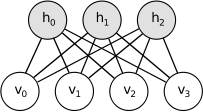
\includegraphics[width=\columnwidth]{rbm.png}}}
% \caption{DBN with one visible layer and one hidden layer}
% %\label{fig:example}
%\end{figure}

\section{related work}
During the past decade, deep learning has been considered by the machine learning community to be one of the most interesting and intriguing research topics. Deep architectures promise to remove the necessity of custom-designed and manually selected features as neural networks should be more powerful in disentangling interacting factors and thus be able to create meaningful high-level representations of the input data. Generally speaking, deep learning combines deep neural networks with an unsupervised learning model. Two major learning models are widely used for this purpose: Restricted Boltzmann Machines (RBMs) and Sparse Auto Encoders. A deep architecture comprises multiple stacked layers based on one of these two models. These layers can be trained one by one, a process that is referred to as ``pre-training'' the network. In this work, we employ RBMs to pre-train the deep architecture in an unsupervised fashion; this is called a Deep Belief Network (DBN). DBNs, composed of a stack of RBMs, essentially share the same topology with general neural networks: DBNs are generative probabilistic models with one visible layer and several hidden layers \cite{hinton2006fast}. 

Since Hinton proposed a fast learning algorithm for DBNs \cite{hinton2006fast}, it has been widely used for initializing deep neural networks. In deep structures, each layer learns relationships between units in lower layers. With the number of RBM layers increasing the complexity of the system increases, making the structure, theoretically, more powerful. An extra softmax output layer can be added to the top of the network (see \eqnref{softmax}); its output can be interpreted as the likelihood of each class.\footnote{add reference!}

LeCun formulated the idea of applying the Convolutional Neural Networks (CNNs) to images as well as speech and other time-series signals \cite{lecun1995convolutional}. This approach, allows to deal with the variability in time and space to a certain degree; CNNs can be seen as a special kind of neural network in which the weights are shared across the input within a certain spatial or temporal area. Therefore, it reduces the overfitting problem due to the weight sharing. The weights thus act as a kernel filter applied to the input. CNNs have been particularly successful in image analysis. For example, Norouzi et al.\ used Convolutional RBMs to learn shift-invariant features \cite{norouzi2009stacks}. 
%\begin{figure}
% \centerline{\framebox{
% 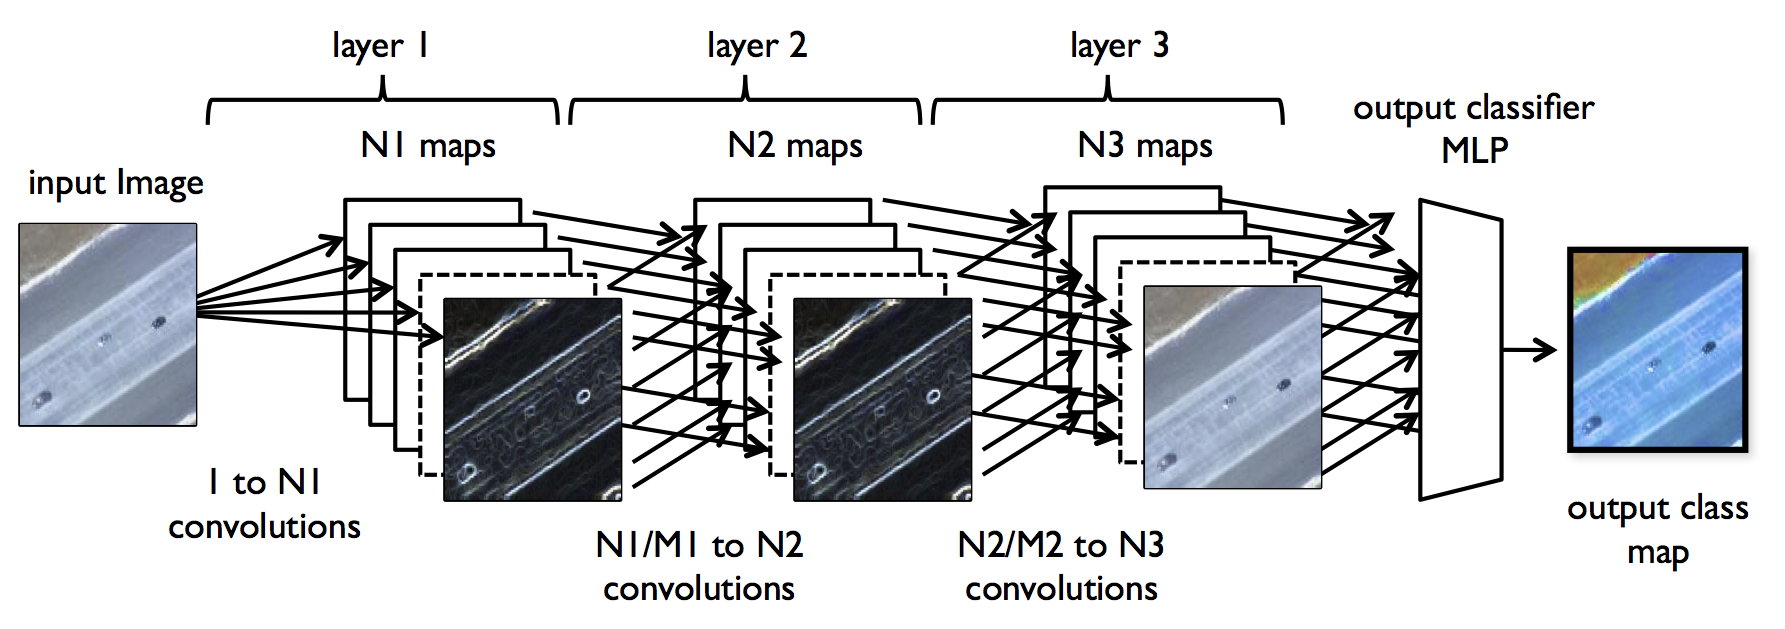
\includegraphics[width=\columnwidth]{neuralnet.png}}}
% \caption{CNNs used for image classification}
% \label{fig:cnn}
%\end{figure}

Modifications of the network architecture obviously result in different results. Grezl et al.\ used a so-called bottleneck architecture neural network to obtain features for speech recognition and showed that these features improve the accuracy of the task \cite{grezl2007probabilistic}. The principle behind the bottleneck-shaped architecture is that the number of neurons in the middle layer is lower than in the other layers as shown in Fig.~\ref{fig:bottleneck}.

Recently, more researchers investigated deep learning in the context of MIR. Lee et al.\ pioneered the application of convolutional deep learning for audio feature learning \cite{lee2009unsupervised}. Hamel et al.\ used the features learned from music with a DBN for both music genre classification and music auto-tagging \cite{hamel2010learning}; their system was successful in MIREX 2011 with top-ranked results. Battenberg employed a conditional DBN to analyze drum patterns \cite{battenberg2012analyzing}. The use of deep architectures for chord detections, however, has not yet been explored, although modern neural networks have been employed in this field. For instance, Boulanger et al.\ investigated recurrent neural networks \cite{boulanger2013audio} and Humphrey has explored CNNs \cite{humphrey2012rethinking,humphrey2012learning}. While they also used the concept of pre-training, their architectures have only two or 3 layers and thus cannot be called ``deep''.
\begin{figure}
 \centerline{\framebox{
 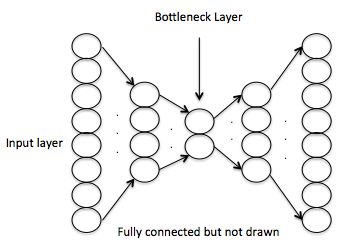
\includegraphics[width=\columnwidth]{bottleneck}}}
 \caption{Bottleneck Neural Network Architecture}
 \label{fig:bottleneck}
\end{figure}

The basic buildings blocks of most modern approaches to chord detection can be traced back to two influential publications: Kawakami proposed to use HMMs for representing chords as hidden states and to model the transition probability of chords \cite{kawakami2000hidden} and Fujishima introduced pitch chroma vectors extracted from the audio as input feature for chord detection \cite{fujishima1999realtime}. Since then there have been a lot of studies using chroma features and HMMs for chord detection\cite{papadopoulos2007large,cho2010exploring}. Examples for recent systems are  Ni, using genre-independent chord estimation method based on HMM and chroma features \cite{ni2012using} and Cho used multi-band features and a multi-stream HMM for chord recognition \cite{cho2013mirex}. Training HMMs with pitch chroma features arguably is the standard approach for this task and the progress is less marked by major innovations but by optimizing and tuning specific components. 

%In this work, we employ deep learning to come up with a novel system for chord detection. 

%\begin{figure}
% \centerline{\framebox{
% \includegraphics[width=\columnwidth]{1.png}}}
% \caption{Underlying chord states from melody}
% %\label{fig:example}
%\end{figure}

\section{System Overview}
Figure~\ref{fig:overview} gives an overview of all components and processing steps of the presented system. The following section will discuss all of these steps in detail.
\begin{figure}
 \centerline{\framebox{
 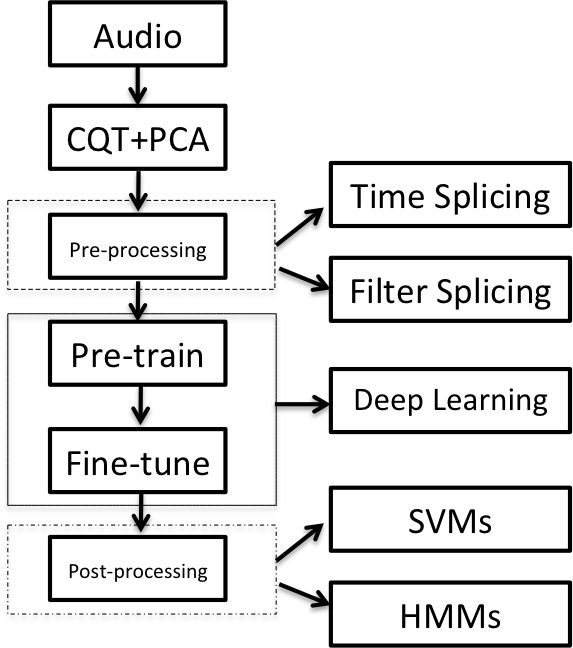
\includegraphics[width=\columnwidth]{flowchart.png}}}
 \caption{The overview of our system}
 \label{fig:overview}
\end{figure}

\subsection{Input Representation}\label{sec:input}
The input audio are converted to a sample rate of \unit[11.025]{kHz}. Then, a Constant Q transform (CQT) is applied. 
The CQT is a perceptually inspired time-frequency transformation for audio. The resulting frequency bins are equally spaced on a logarithmic (``pitch'') scale. It has the advantage of providing a more musically and perceptually meaningful spectral representation than the DFT. 
We used an implementation of the CQT as a filterbank of Gabor filters, spaced at \unit[36]{bins per octave}, i.e.\ \unit[3]{bins per semitone}, yielding \unit[180]{bins} representing a frequency range spanning from \unit[110]{Hz} to \unit[3.520]{kHz}. Finally, we use Principal Component Analysis (PCA) for decorrelation, and apply Z-Score normalization\cite{sola1997importance}. 

\subsection{Pre-Processing}\label{sec:pre-proc}
Neighboring frames of the input representation can be expected to contain similar content, as chords will not change on a frame-by-frame basis. In order to take into account the relationship between the current frame and previous and future frames, we investigate the application of several pre-processing approaches.

\subsubsection{Time Splicing}
Time splicing is a simple way extend the current frame with the data of neighboring frames by concatenating the frames into one larger superframe. For example, assuming there are 7 input frames. In first order time splicing, we concatenate the current frame, the previous frame, and the following frame. Thus, the 4th superframe is comprised of the 3rd, 4th, and 5th frame. Since the same operation will be applied for the 5th superframe etc., there will be overlap introduced between neighboring superframes. %We conduct such operation along over all frames in each piece with different splice amount. 
%\begin{figure}
% \centerline{\framebox{
% 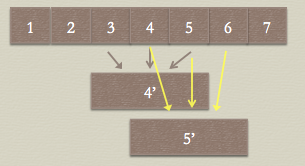
\includegraphics[width=\columnwidth]{timesplice}}}
% \caption{Illustration for time splicing}
% \label{fig:splicing}
%\end{figure}

\subsubsection{Convolution}
Although we do not use CNNs, we employ a pre-processing step inspired by CNNs. Essentially, CNNs have one or more convolutional layers between the input and lower layers of the neural network. The function of a convolutional layer can be interpreted as the application of a linear filter plus a non-linear transformation, sometimes also combined with pooling operation:
\begin{equation}\label{Covulution}
Y = \pool(\sigm(K \ast X + B)), 
\end{equation}
in which $Y$ is the output of a convolutional layer, $K$ is the linear kernel filter (impulse response), $X$ is the input, $B$ is the bias, $\sigm()$ is a non-linear transform, and $\pool()$ is a down-sampling operation. The uniqueness of convolutional networks stems from the convolution operation applied to the input $X$. We emulate this functionality by applying filters to the input signal. Instead of learning the filters, we manually design several filters.
%Instead of training the filters automatically, we can make use of the prior knowledge to design the filters manually. In the case of chord detection, given we mainly want to extract time information by convolution, so we design time domain filters. \\

An obvious choice are low pass filters. 
We employ a simple single pole low pass filter due to its easy parameter configuration. Given that our system is not required to work in real-time, we can apply anti-causal filtering and filter the signal in both directions so that the resulting overall filter has a zero phase response (compare the Matlab function \verb1filtfilt1).

%Under the assumption that the frame that is located in the middle of a chord is way more obvious and easier to be detected than the frame that is located at the boundary of a chord, w
We also apply two other low pass filters, both of which have exponential decay shaped impulse response. The difference equations are given in \eqnref{filter1} and \eqnref{filter2}. 
\begin{equation}\label{filter1}
y_{1}(n) = \sum_{k=1}^N a^{-k+1} x(n-N+k)
\end{equation}
\begin{equation}\label{filter2}
y_{2}(n) = \sum_{k=1}^N a^{-k+1} x(n+N-k)
\end{equation} 
The filter length is $N$ and $a$ is the exponential base. 
These filters are not centered around the current frame anymore, but shifted by $N$ frames. Their impulse responses are symmetric to each other. One could interpret these filters as to focus on past frames and future frames, respectively. We will refer to these filters as ``extension filters". 

The ideas of splicing and convolution can be combined, as exemplified by Fig.~\ref{fig:filtersplice}.
%In a further processing, we combine the ideas of time splicing and convolution: we either conduct time splicing on the output of the low pass filter, or splice the output of different filters together, as in figure 4.
\begin{figure}
 \centerline{\framebox{
 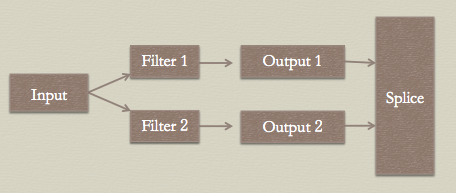
\includegraphics[width=\columnwidth]{CNN}}}
 \caption{Splicing output of different filters}
 \label{fig:filtersplice}
\end{figure}
We call this kind of processing as ``splice filtering. 
 
\subsection{Training}\label{sec:train}
It is impractical to train DNNs directly with back propagation using gradient decent due to their deep structure. Therefore, the network is usually initialized by an unsupervised pre-training step. As our network consists of RBMs, Gibbs sampling can be used for training. The objective is to retain as much information as possible between input and output. 

The computation between layers can be represented as:
\begin{equation}\label{dbn}
Y_{l} = \sigm(W_{l}X_{l} + B_{l}) ,
\end{equation}  
which is identical to many traditional neural networks. Therefore, a standard back propagation can be applied after pre-training to fine-tune the network in a supervised manner. The loss criterion we use in this work is cross-entropy.  

\subsection{Architecture}\label{sec:arch}
We investigate a deep network with $6$ layers in two different architectures. The common architecture features the same amount of neurons in every layer, in our case $1024$. The bottleneck architecture has a lower number of neurons in the middle layers, namely $256$ neurons in the middle layer, $512$ in its neighboring layers, and $1024$ neurons in the remaining layers\cite{grezl2007probabilistic}.
A softmax output layer is stacked on top of both architectures as described by \eqnref{softmax}.\footnote{maybe move this to related work??}
\begin{equation}\label{softmax}
\softmax(Y_{l}) = \frac{\exp(Y_{l})}{\sum_{k=1}^N \exp(Y_{k})}
\end{equation}
Our network is implemented using the Kaldi package developed by John Hopkins University \cite{povey2011kaldi}.
 
\section{Classification}\label{sec:class}
The output of the softmax layer can be interpreted as the likelihood of each class; taking the maximum will provide a class decision (this method will be referred to as \textit{Argmax}). Alternatively, the output can be treated as intermediate feature vector that can be used as an input to other classifiers for computing the final decision. 
\subsection{Support Vector Machine}
Support Vector Machines (SVMs) are as a widely used classifier with generally good performance an obvious choice. The SVM is trained using the output of the network as features, and the classification is carried out for every frame. The classification is followed by a simple prediction smoothing.
\subsection{Hidden Markov Model}
HMMs are, as pointed out above, a standard classifier for automatic chord detection because the characteristics of the task fit the HMM approach well: Chords are hidden states that can be estimated from observations (feature vectors extracted from the audio signal), and the likelihood of chord transitions can be modeled with transition probabilities. 
Modified HMMs such as ergodic HMMs and key-independent HMMs have been also explored for this task \cite{papadopoulos2007large,lee2008acoustic}. In this work we are mostly interested in the performance comparison between different features, so a simple first-order HMM is used. 
Given the probabilistic property of softmax output layer, we can use it directly as emission probabilities in the context of HMMs. Therefore, there is no need to train the HMM using, e.g., the commonly used Baum-Welch algorithm. Instead, the histogram of each class in our training is used as initial probabilities, and the bigram of chord transitions is used to compute the transition probabilities. Finally, we employ the Viterbi decoding algorithm to find the globally optimal chord sequence. 

\section{Evaluation procedure}
\subsection{Dataset}
Our dataset is a combination of several different datasets, yielding a 311-piece collection. The data is composed of 
\begin{itemize}
	\item   $180$ songs from the \textit{Beatles dataset} \cite{},
    \item   $100$ songs from the \textit{RWC Pop dataset} \cite{}, 
    \item   $18$ songs from the \textit{Zweieck dataset} \cite{}, and 
    \item   $13$\footnote{I thought it was 31 labeled songs in the queen dataset? Double check all numbers!} songs from \textit{Queen dataset} \cite{}.
\end{itemize}  
The pre-processing as described in Sect.~\ref{sec:pre-proc} ensures identical input audio formats.

\subsection{Methodology}

The dataset is divided randomly into two parts: 80\% for the training set and 20\% for the test set. Within the training set, 10\% of the data is used as a validation set. \footnote{How is training and test data used between training the network and training the post classifiers??}

The chosen outputs for classification are major and minor triads for every root note, resulting in a dictionary of $24+1$ chord labels.
Ground truth time-aligned chord symbols are mapped to this major/minor dictionary:\footnote{are you sure that this equation helps anyone? I feel it's more confusing than helping. And what is C? The dictionary?}
\begin{equation}
C_{majmin} \subset {N} \cup S \times {maj,min}
\end{equation}
with $S$ representing the 12 pitch classes (root notes) and $N$ being the label for unknown chords. In the calculation of the detection accuracy, the following chord types are mapped to the corresponding triads in the dictionary: triad major/minor and seventh major/minor. Other chord types are treated as unknown chords. For instance, G:maj and G:maj7 are mapped to `G:maj'; G:dim and G:6 are all mapped to `N'.\footnote{Maybe it is worth noting here how the ground truth is distributed after this procedure? Most importantly the probability of the largest class?}

\subsection{Evaluation Metric}
The used evaluation metric is the same as proposed in the audio chord detection task for MIREX 2013: the Weighted Chord Symbol Recall (WCSR) is used to estimate how well the predicted chords match the ground truth. WCSR, formulated in \eqnref{csr}, is defined as the total duration of segments with correct prediction: \footnote{verify that this is correct --- sounded to like it as the CSR divides byt the song length and the WCSR weights with the song length...}  
\begin{equation}\label{csr}
WCSR = \frac{1}{N} \sum_{k=1}^n TP_{k},
\end{equation}
in which $n$ is the number of test samples (songs), $N$ is the total number of frames in all test samples, and $TP_{k}$ is the number of frames that are correctly detected in the kth sample. 

\section{Experiments}

\subsection{Learning strategies}
There are three different training scenarios:
\begin{itemize}
	\item   unsupervised training (the trained network will be referred to as $DN_\mathrm{DBN}$)
	\item   supervised training (the trained network will be referred to as $DN_\mathrm{DNN}$)
    \item   the combination of unsupervised (pre-training) and supervised (fine-tuning) training  (the trained network will be referred to as $DN_\mathrm{DBN-DNN}$)
\end{itemize} 
In this experiment, no pre-processing is applied to the data; the input is simply the input representation (CQT followed by PCA) as described in Sect.~\ref{sec:input}. The chosen architecture for this experiment is the bottleneck architecture.
As the $DN_\mathrm{DBN}$ scenario is unsupervised, we take the output of bottleneck layer as input to the classifier, in this case an SVM. For the $DN_\mathrm{DNN}$ (supervised but no pre-training), back propagation is used to train the neural network and an HMM with Viterbi decoding is used for classification. Finally, in the case of the $DN_\mathrm{DBN-DNN}$ (pre-training and supervised learning), three different classifiers are compared: the maximum of the softmax output (Argmax), an SVM, and an HMM. 
\begin{table}
\centering
\begin{tabular*}{\columnwidth}{@{\extracolsep{\fill}}llr}
%\begin{tabular}{@{}llr@{}}
\toprule
\textbf{Training Scenario} & \textbf{Classifier} & \textbf{WCSR}  \\ \hline
$DN_\mathrm{DBN}$             & SVM            & 0.141 \\ 
$DN_\mathrm{DNN}$              & HMM            & 0.159      \\ 
$DN_\mathrm{DBN-DNN}$         & Argmax()            & 0.648 \\ 
$DN_\mathrm{DBN-DNN}$          & SVM            & 0.645 \\ 
$DN_\mathrm{DBN-DNN}$         &  HMM           & \textbf{0.755} \\ \hline
\end{tabular*}
\caption{Chord detection performance of different learning strategies}
\label{dbn-dnn}
\end{table}

Table \ref{dbn-dnn} lists the results of the experiment. It comes as no surprise that the combination of unsupervised and supervised training ($DN_\mathrm{DBN-DNN}$) greatly outperforms both the unsupervised $DN_\mathrm{DBN}$ and the supervised $DN_\mathrm{DNN}$ training scenarios. In the comparison between the three output classifiers, the HMM performs best, while there is only minimal distance between the Argmax and SVM output.

\subsection{Filters Evaluation}
As stated in previous section, we investigate to design different filters in pre-processing. The first type is linear phase signal pole filter, the difference equation is formulate as \eqnref{IIR}:
\begin{equation}\label{IIR}
y_{n} = (1-\alpha) y_{n-1} + \alpha x_{n}
\end{equation}
Normally, the IIR filters do not have a linear phase response. But we use filtfilt technique to achieve zero phase. Noting that there is only one parameter $\alpha$ which determines the frequency response shape. We conduct a grid search for this parameter, starting from 0.25 to 0.75 with the step size of 0.25. Meanwhile we compare it with different five-order FIR low-pass filter centered around the current frame. The FIR coefficients are exponentially decreased in both side, ie. the impulse response is in Laplace shape. Furthermore, we also combine the ideas of convolution and time splicing. We concatenate the output of low-pass filter together as time splicing does. Inspired by CNNs, we can also concatenate the output of different filters, the results are shown in figure 5.

\begin{figure}
 \centerline{\framebox{
 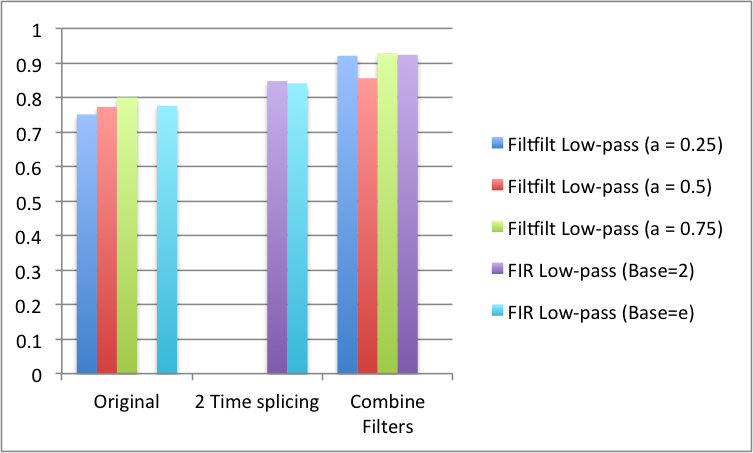
\includegraphics[width=\columnwidth]{filters.png}}}
 \caption{Comparison Between different filters}
 %\label{fig:example}
\end{figure}

\subsection{Architecture}
\subsubsection{Common vs. Bottleneck}
As mentioned before, we employ a bottleneck architecture in this work. According to \cite{grezl2007probabilistic}, deep networks are suitable in a bottleneck architecture to learn high-level features. We can consider the bottleneck networks as two halves. The first half is from the first layer to the bottleneck layer, in which the number of neurons gradually decreases. This is actually an encoding or compression process. The useful information gets compacter as well as the redundant information can be gotten rid of. The second half is from the bottleneck layer to the last layer, in which the number of neurons gradually increases. We can see it as a decoding process. By these two processes, the networks are able to extract the useful information and discard the redundant ones. Another benefit of bottleneck architecture is that it can reduce the overfitting issue by decreasing the complexity of the system. We compare the common architecture and the bottleneck architecture under the same configurations. In comparison, the configurations are: HMMs as post-classifiers; DBN-DNNs as training strategy. The results are listed in table 2.

% Please add the following required packages to your document preamble:
% \usepackage{booktabs}
\begin{table}[h]
\begin{tabular}{@{}cccc@{}}
\toprule
Architecture                   & Pre-processing                      & \begin{tabular}[c]{@{}c@{}}Training\\ WCSR\end{tabular} & WCSR  \\ \midrule
Common                         & None                                & 0.843                                                      & 0.703 \\
Bottleneck                     & None                                & 0.855                                                      & 0.755 \\
Common                         & 2 Time Splicing                     & 0.903                                                  & 0.712 \\
\multicolumn{1}{l}{Bottleneck} & \multicolumn{1}{l}{2 Time Splicing} & 0.892                                 & 0.821 \\ 
Common     & Splice Filtering & 0.985 & 0.876 \\
Bottleneck & Splice Filtering & 0.936 & 0.919 \\ \bottomrule
\end{tabular}
\caption{Chord detection performance of different architecture}
\end{table}

\subsubsection{Single-Label vs. Multi-Label}
Because of the hierarchical property of chords, our learning targets are not limited to chords themselves. Since chords can be decomposed into pitches, therefore we could let the networks learn pitch information instead of chords. By doing so, we hope it can decrease the abstraction and complexity of the task. The main reason for that is pitches are more directly related to the input representations, ie. CQT. It will, however, lead to another issue which is we will transfer the single target learning task to multi-target learning. We use several settings based on the previous experiments to conduct the comparison between chords and pitches. The results are listed in table 4. 

\begin{table}[h]
\begin{tabular}{@{}cccc@{}}
\toprule
Learning Targets & Pre-processing   & \begin{tabular}[c]{@{}c@{}}Post-\\ processing\end{tabular} & WCSR  \\ \midrule
25 Chord Classes & Splice Filtering & Viterbi                                                    & 0.919 \\
12 Pitch Classes & Splice Filtering & HMMs                                                       & 0.78  \\ \bottomrule
\end{tabular}
\caption{Chord detection performance of different learning targets}
\end{table}
As seen from the results, learning pitches does not really work. There should be several potential reasons. Even though we believe the idea of decomposing chords will bring some benefits, some practical issue may impact such benefits: firstly, multi-target learning is relatively more difficult for the model per se to train. Since in our implementation of multi-target training, we assign each target a equal posterior, which is less obvious than the single target for models to learn. Second, in the real audio files, some notes are occasionally removed from or added into a chord, which could make the pitch ground truth inaccurate. Therefore, we give up this idea in our final evaluation. 

\section{Results}
\subsection{Results}
From previous discussions and comparisons, several settings show the most promise. So we decide to use them as the default configuration in our final evaluations: bottleneck structure outperforms the common structure both in accuracy and time-complexity; DBN-DNNs training strategy beats DBNs and DNNs training strategies without much surprise; splice filtering similar to what CNNs do, generally speaking, yields a better result than the others; finally, Viterbi decoding as post classifiers are more appropriate for this task due to the dynamic properties of chords.  \\
In previous published results \cite{cho2011feature} on the similar dataset is around 80\%. We present the mean accuracy of 3 fold cross-validation obtained on our 311-piece dataset at the major/minor level (total 25 classes). We compare our results with Chordino approach on our dataset, though in an unfair way, as baseline system. Noting that Chordino system can not only detect major/minor scale, it can detect as much as 120 different chords. Thus we map the Chordino results into our major/minor scale. In this mapping, due to the different chord annotation rules, we could make mistakes through imperfect parsing. The results are listed in table 4, in which Type1 pre-processing is to splice the 5-order FIR low-pass filter and extension filters; whereas Type2 pre-processing is to splice the single-pole IIR low-pass filter and extension filters. 

% Please add the following required packages to your document preamble:
% \usepackage{booktabs}
\begin{table}[h]
\begin{tabular}{@{}ccc@{}}
\toprule
Methods   & Pre-processing & WCSR   \\ \midrule
Chordino & N/A            & 0.625       \\
Proposed DBN-DNNs & Type1          & 0.911 \\
Proposed DBN-DNNs & Type2          & 0.919   \\ \bottomrule
\end{tabular}
\caption{Chord detection performance of different methods}
\end{table}

\subsection{Discussion}
We presented a comprehensive system for chord detection, that is competitive with the existing start-of-the-art systems. Our DBN-DNNs model can learn a high-level probabilistic representations for chords. The Viterbi algorithm is applied to find a global optimal path based on the output of our DBN-DNNs as the predicted chord sequence. Furthermore, the bottleneck structure have a stronger learning ability for chords information than the common architecture. By the process of ``encoding" and ``decoding", the networks retain the ``essential information" but discard the redundant ones. The results also indicate that applying pre-processing will significantly increase the accuracy. That's because it will introduce temporal continuity and dynamics into feature representation. Intuitively, dynamic programming algorithms such as Viterbi decoding outperforms the static classifiers such as SVMs due to the dynamic property of chords. Therefore introducing transition probability makes more sense. 

\section{Conclusion}
In this work, we present a system which applies deep learning to the chord detection task. Our DN model is able to learn the high-level features for chord detection across various configurations. Combined with the appropriate pre-processing and post-processing, the performance can compete with state-of-the-art systems. Our pre-processing methods can retain temporal continuity and dynamics in our features; our post-processing could take care of the high-level musical context information. With a bottleneck structure, the overfitting issue s significantly reduced. With some practical limitations, multi-target training using pitch information does not work as well as single-target counterpart. The idea is, however, promising and worthy exploring in the future works. 

\bibliography{ISMIR2015template}
\end{document}
